% Guide de lecture du calcul ; aucun paramètre ni résultat supplémentaire.
\begin{figure}[H]
\centering
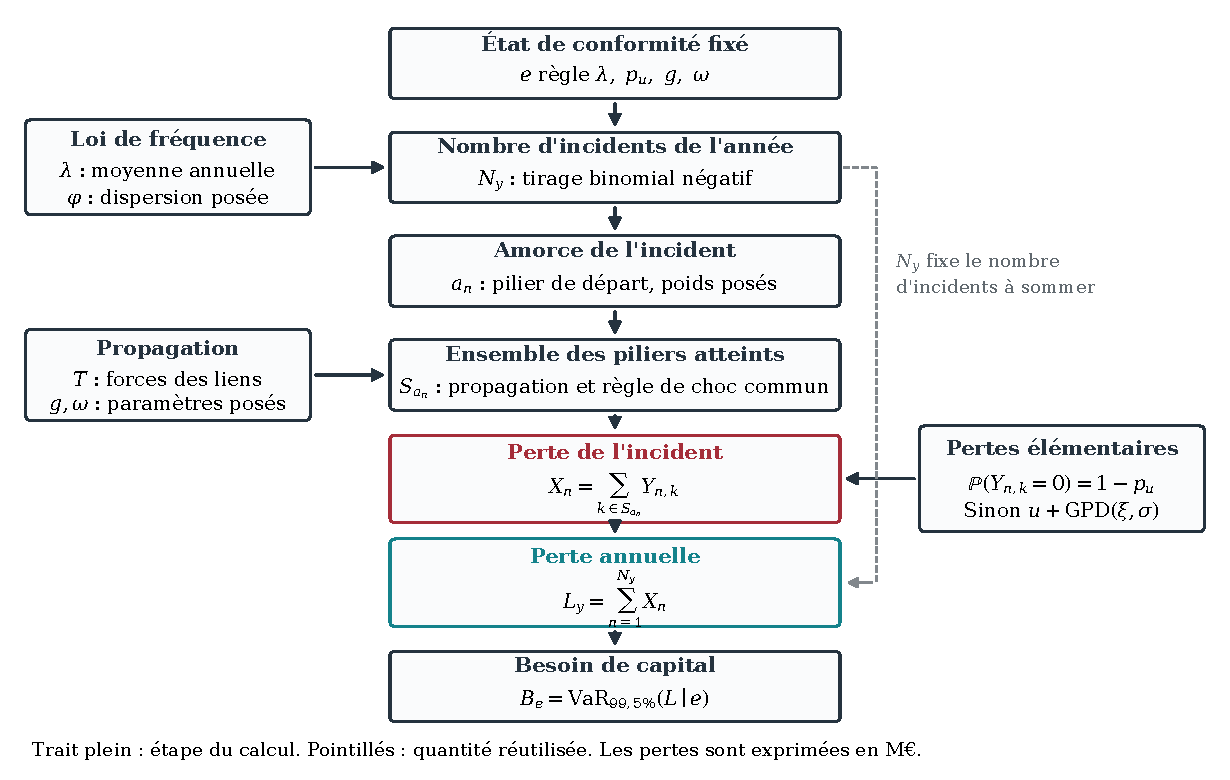
\includegraphics[width=\textwidth]{figures_pedagogie/flux_perte_annuelle.pdf}
\caption{Flux de calcul d'une perte annuelle à état fixé. $y$, $n$ et $k$ indexent l'année simulée, l'incident et le pilier. $u$ est le seuil monétaire ; $\xi$ et $\sigma$ sont la forme et l'échelle de la GPD. Le chapitre~\ref{chap:cascade} détaille la loi des ensembles atteints.}
\label{fig:lecture-architecture}
\end{figure}

Reprenons l'incident de l'introduction : il part de P4 et touche P1 puis P2. Si ses pertes
élémentaires sont $a$, $b$ et $c$, sa contribution à l'année vaut $a+b+c$ sous la règle additive.
Les pertes des autres incidents de cette année s'y ajoutent pour former $L_y$.
Le capital est un quantile des sommes $L_y$ répétées en simulation ; ce n'est pas le quantile
de $a+b+c$ seul. Les branches latérales indiquent les paramètres des étapes. Le tableau~\ref{tab:chaine-calcul}
en précise les sources et le statut, puis indique ce qui change pour une entité.

\begin{table}[htbp]\centering\small
\renewcommand{\arraystretch}{1.18}
\begin{tabularx}{\textwidth}{@{}p{.15\textwidth}>{\raggedright\arraybackslash}X>{\raggedright\arraybackslash}X>{\raggedright\arraybackslash}p{.24\textwidth}@{}}
\toprule
\textbf{Étape} & \textbf{Entrée} & \textbf{Sortie} & \textbf{Statut} \\
\midrule
Données & pertes SAS OpRisk cyber $\times$ finance ; parts Hackmageddon & $\lambda$, $u$, $\xi$, $\sigma$, $p_u$ ; parts $\pi_v$ & estimés (ch.~\ref{chap:donnees} et~\ref{chap:socle}) ; $\pi_v$ cité \\
État & multiplicateurs, détection, $g$, $\omega$ & valeurs des quatre canaux par état & posés (\S\ref{sec:quatre-canaux}) \\
Incident & amorce, matrice $W$, gain $g$ & ensemble atteint, somme des pertes de ses piliers & $W$ posée ; direction non identifiée (ch.~\ref{ch:identifiabilite}) \\
Année & nombre $N_y$, binomiale négative de surdispersion $\varphi$ & charge annuelle $L_y$ & $\varphi$ posé \\
Quantile & charges annuelles simulées & besoin $B=\VaR_{99{,}5\,\%}(L)$ & bruit de simulation publié \\
Entité & panel d'entités, élasticités de fréquence et de sévérité & besoin $B(A)$, cascade indépendante sans choc P4 & élasticité de sévérité estimée ; $b_\lambda$ estimé sur les grandes institutions, extrapolé (\S\ref{sec:ancrage}) \\
\bottomrule
\end{tabularx}
\caption{La chaîne de calcul, étape par étape. Les étapes Incident à Quantile sont celles de la
figure~\ref{fig:lecture-architecture} ; l'étape Entité change de moteur.}
\label{tab:chaine-calcul}
\end{table}
